
\centering
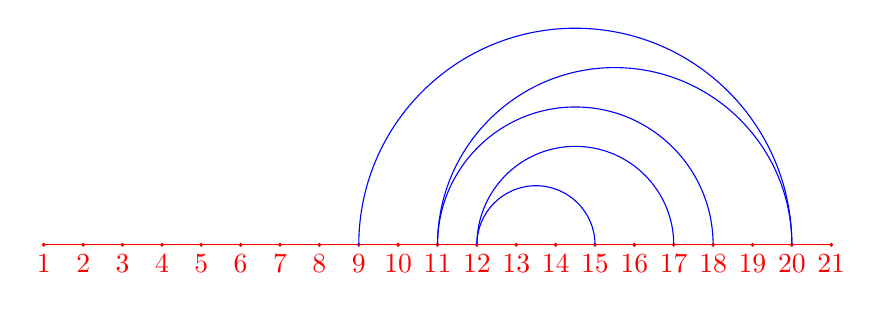
\begin{tikzpicture}[scale=0.5]


\foreach \i in {1,...,20} {
        \draw[red] (\i,1) -- (\i + 1,1)node[pos=0.0,below] {\i};
        \filldraw[red] (\i,1) circle (1pt);


 }

\draw[red] (21,1) -- (20,1)node[pos=0.0,below] {21};
\filldraw[red] (21,1) circle (1pt); 



\draw[blue, thin] (9,1) arc(180:0:5.5); 
\draw[blue, thin] (11,1) arc(180:0:4.5); 
\draw[blue, thin] (11,1) arc(180:0:3.5); 
\draw[blue, thin] (12,1) arc(180:0:2.5);
\draw[blue, thin] (12,1) arc(180:0:1.5);
\end{tikzpicture} 